\documentclass[defaultstyle,11pt]{thesis}

\usepackage{amssymb}		% to get all AMS symbols
\usepackage{amsmath}		% to get equations to work right
\usepackage{graphicx}		% to insert figures
\graphicspath{{../}{Trap/}}
\usepackage[pagebackref = true]{hyperref}		% PDF hyperreferences?? [backref=none]
\usepackage{natbib}
\usepackage{array}
\newcolumntype{L}[1]{>{\raggedright\let\newline\\\arraybackslash\hspace{0pt}}m{#1}}
\newcolumntype{C}[1]{>{\centering\let\newline\\\arraybackslash\hspace{0pt}}m{#1}}
\newcolumntype{R}[1]{>{\raggedleft\let\newline\\\arraybackslash\hspace{0pt}}m{#1}}
\usepackage{caption}
\setcitestyle{numbers,square,comma}
\usepackage[usenames,dvipsnames]{color}
%% To make \href colors more decent:
\definecolor{MyDarkBlue}{rgb}{0,0.1,0.7}
\hypersetup{pdfborder={0 0 0},colorlinks,breaklinks=true,
  urlcolor={MyDarkBlue},citecolor={MyDarkBlue},linkcolor={MyDarkBlue}
}
\renewcommand{\thefootnote}{\alph{footnote}}	
\title{a}
\abstract{a}
\author{a}{a}
\otherdegrees{a}
\degree{a}{a}
\dept{a}{a}
\advisor{a}{a}
\reader{a}
\readerThree{a}
\SuspendPrologue
\begin{document}

\newtheorem{theorem}{Theorem}


\newcommand{\diff}[2]{\frac{\partial #1}{\partial #2}}
\newcommand{\diffr}[1]{\diff{#1}{r}}
\newcommand{\diffth}[1]{\diff{#1}{\theta}}
\newcommand{\diffz}[1]{\diff{#1}{z}}

\newcommand{\vth}{V_{\theta}}

\newcommand{\twochoices}[2]{\left\{ \begin{array}{lcc}
        \displaystyle #1 \\ \vspace{-10pt} \\
        \displaystyle #2 \end{array} \right. } %}

\newcommand{\threechoices}[3]{\left\{ \begin{array}{lcc}
        #1 \\ #2 \\ #3 \end{array} \right. }    %}

\newcommand{\fourchoices}[4]{\left\{ \begin{array}{lcc}
        #1 \\ #2 \\ #3 \\ #4 \end{array} \right. }      %}

\newcommand{\twovec}[2]{\left(\begin{array}{c} #1 \\ #2 \end{array}\right)}
\newcommand{\threevec}[3]{\left(\begin{array}{c} #1 \\ #2 \\ #3 \end{array}\right)}
\newcommand{\twomatrix}[4]{\left(\begin{array}{cc} #1 & #2 \\ #3 & #4 \end{array}\right)}

% dave's figure shortcut. arguments are 1, a dual label and filename, 2, the short caption for LOF, 3, the long caption, and 4, the width.
\newcommand{\figdave}[4]{
\begin{figure}[t!]
\centering
\vspace{0.5mm}
\includegraphics[width=#4]{#1}
\caption[#2]{#3\label{#1}
}
\end{figure}}

% shortcuts for OH ground state labels
\newcommand{\f}[1]{$|f,\frac{{#1}}{2}\rangle$}
\newcommand{\e}[1]{$|e,\frac{{#1}}{2}\rangle$}
\newcommand{\fm}[1]{$|f,-\frac{{#1}}{2}\rangle$}
\newcommand{\emm}[1]{$|e,-\frac{{#1}}{2}\rangle$}
\newcommand{\fpm}[1]{$|f,\pm\frac{{#1}}{2}\rangle$}
\newcommand{\epm}[1]{$|e,\pm\frac{{#1}}{2}\rangle$}

% I need to add macros from spin flip loss paper to get that part to compile.
\newcommand{\bcl}{{$B_\text{coil}$}}
\newcommand{\epb}{{$\vec{E}\s {\perp}\s\vec{B}$}}
\newcommand{\epbm}{{\vec{E}\s {\perp}\s\vec{B}}}
\newcommand{\cmnt}[1]{\ignorespaces}
\newcommand{\s}{{\nobreak\hspace{.2em}}}


\chapter{Molecular Trapping}

Some of the earliest successful trapping of neutral molecules began with CaH in John Doyle's group in a dilution fridge with $^3$He buffer~\cite{Weinstein1998}.
Stark decelerated and electrostatic trapped ammonia followed soon later~\cite{Bethlem2000trap}.
Since then extensions to many species have occurred. 
In this chapter we focus on OH molecules, whose strong Stark shift to mass ratios make them favorable for attempts to attain high enough densities to observe collisions between members of the ensemble.

\section{History of OH traps}

%Trap History Table
\renewcommand{\arraystretch}{1.5}
\begin{table}[t!]
\centering
\caption{
The Ye Group Molecule trapping endeavor.\label{trappingtable}
}
\label{tab:rates}
\begin{tabular}{ L{2.5cm} | C{4.5cm} C{2.5cm} C{4.5cm} }
Name & Type & Depth (mK) & Uses \\
\hline\hline
MET 	& Magnetic Quadrupole, Electric Hexapole & 250 	& First Demonstration~\cite{Sawyer2007} 	 \\
\hline
Ring 		& Magnetic Quadrupole				& 100 	& He, D$_2$, ND$_3$ Collisions~\cite{Sawyer2008,Sawyer2011} \\
\hline
Ring 		& Above, but new mounts				& 100 	& E-field Induced Collisions,  Evaporation~\cite{Stuhl2012uwave,Stuhl2012evap,Stuhl2013} \\
\hline
Tricycle 	& Magnetic Quadrupole 				& 300 	& 10x density, spin-flip loss \\
\hline
Pin  		& 2D Magnetic and Electric Quadrupoles 	& 500 	& Solved spin-flip loss~\cite{Reens2017}\\
\hline
Cryocycle 	& Magnetic Quadupole 				& 200 	& Lifetime, Fluorescence Enhancements\\
\end{tabular}
\end{table}

The history of OH trapping in the Ye group has grown substantial enough to warrant a tabular environment~\ref{trappingtable}. 
Each attempt has brought new challenges and experiences, and steady progress has been made in a number of key areas.
The Magnetoelectrostatic Trap (MET) installed during Brian Sawyer's time~\cite{Sawyer2007} was a heroic first attempt that included a few-turn magnetic coil run at a startling $1400$~A, and $2000$~A briefly during loading.
Later it was decided to trade the role of the fields used for loading, and great gains in magnetic field strength and simplicity were attained by switching to permanent magnets with the ``Ring'' trap~\cite{Sawyer2011}.
A key improvement occurred when it was discovered that patch charges on the Ultem mounts originally used for affixing the magnetic trap to the Stark decelerator could have a significant impact on spectroscopic efforts~\citep[Fig.~6]{Stuhl2012uwave}.
This was addressed by designing primarily stainless steel mounts, so that molecules only had line of sight to grounded conductors, although still with insulators installed between the decelerator and trap but relocated elsewhere.

\section{Trap Spectroscopy}

\section{Tricycle over Ring Trap}

In pursuit of increases in density and molecule number, an iteration on the Ring trap was performed, dubbed the ``Tricycle'' trap due to the three rectangles formed when examining planar cuts through the ring and rear magnets used to generate the trap, see Fig.~\ref{ringtricyclefigure}.
This was first installed in 2014, and improved on the Ring trap in several key ways:
\begin{enumerate}
\item Replaced rear ring with its core, removing an outer toroidal trap and tripling depth.
\item Significantly improved loading dynamics.
\item Increased trap gradient, thanks to a $\sim 40\%$ reduction in size.
\end{enumerate}

\begin{figure}[t!]
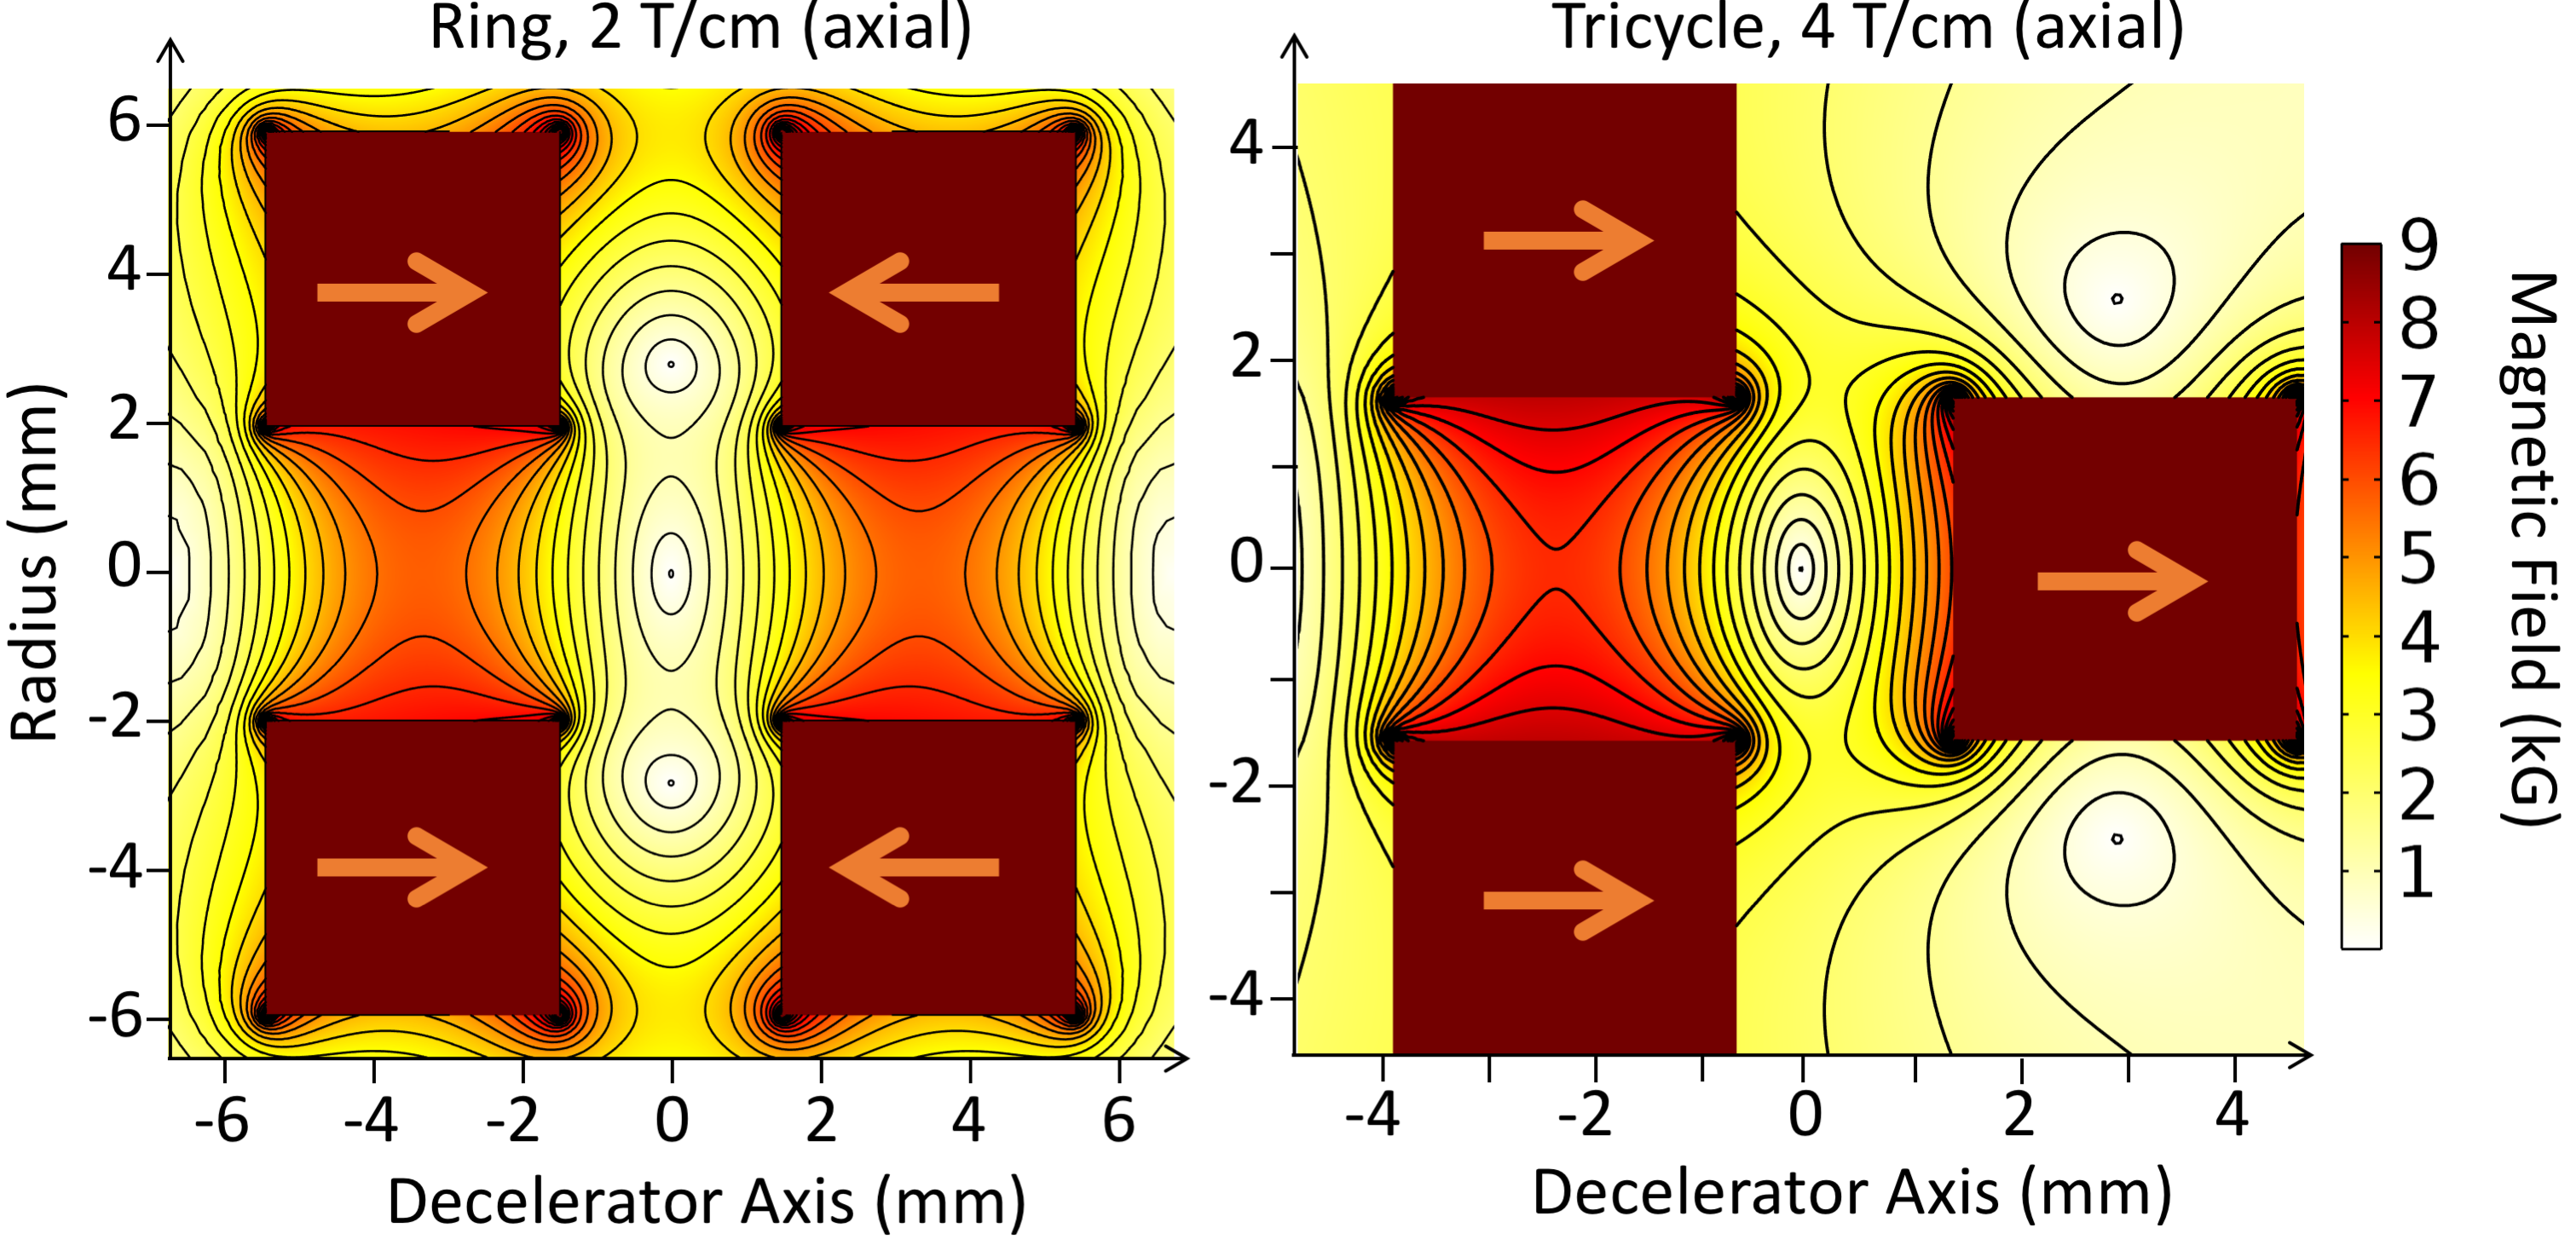
\includegraphics[width=\linewidth]{RingTricycle.png}
\caption[Ring and Tricycle Trap Comparison]{\label{ringtricyclefigure}
Cross Sections including the cylindrically symmetric axis for both the Ring and Tricycle traps. Arrows indicate magnetization directions up to an overall sign. Magnetic trapping fields are shown, demonstrating the destabilization of the toroidal minimum of the Ring trap. Contours every $500$~G. Steel mounting electrodes are not shown in either case, but are installed on the outer diameter of the magnets and affixed to them with setscrews.
}
\end{figure}

\subsection{Toroidal Destabilization}

This first achievement was one of the primary goals of the iteration, since the influence of the toroidal minimum present in the Ring trap was difficult to ascertain. 
Molecules ought to have been able to explore the toroidal region, but based on the observed distribution of molecules as a function of magnetic field, they did not appear to be doing so for unknown reasons.
The twofold increase in trap gradient would correspond to an eightfold increase in density, if the same initial temperature were obtained.

\subsection{Loading Improvements}

The Tricycle trap features very significant loading improvements over the Ring trap, although the precise extent is difficult to pin down. 
The main reason for an expectation of improvement lies in the phase space dynamical behavior of the two geometries.
In analyzing any trap loading scenario, it is important to pursue the analysis with both intuition and simulation.
The latter on its own will lack the guidance necessary for truly identifying an optimal scenario, while the former is unlikely to be able to fully disentangle interdependent factors influncing performance.

On the intuitive side, it is useful to use the same reasoning as in the decelerator by focusing on phase stability.
The loading fields generated by charging up the surfaces of the ring magnets in the Ring trap are mirror symmetric about the center of the Ring trap.
This means that if a loading sequence is designed so that the synchronous molecule ends up exactly in the trap center, the synchronous molecule will be required to roll up to the top of a hill and then stop there. 
Molecules with slightly more forwards velocity than the synchronous molecules will end up quite a ways down the other side of the hill by the time the loading fields are switched off, and vice versa.
In layman's terms, longitudinal phase stability during loading requires that the loading be performed on a slope, not a peak.

It is possible to generalize these ideas further, while still remaining in the intuitive domain.
If it is true that the loading fields ought to feature a slope at the location of the trap center where the synchronous molecule comes to rest, what is the ideal value for that slope?
Also, is there a similar ideal value for the slope of the loading fields in the region in front of and beyond the trap center?
We can answer these questions with a simplified thought experiment, refer to Fig.~\ref{LoadingRotation}.
Suppose we have a population experiencing a harmonic trapping potential with a characteristic width $\delta z$ in real space and $\delta v$ in velocity space, and centered at $z_0=0$ and $v_0 > 0$.
One way to controllably transfer this population to $v_0=0$ without unwanted stretching of the population would be to load it into a much larger harmonic potential with oscillation frequency $\omega$ centered at $z=0$ and $v=0$.
Because harmonic potentials always execute rotations in phase space with ellipticity controlled by their oscillation frequency, the population would then be smoothly transferred over the course of a quarter oscillation to be centered at $z = v_0/\omega$ and $v=0$, with widths $\omega\delta z$ and $\delta v/\omega$.
If $\omega$ is chosen equal to $\delta v/\delta z$, i.e. to have the same strength as the trapping potential prior the initiation of the loading sequence, then the original widths in position and velocity are precisely maintained.
On the other hand, $\omega$ could be tuned so as to optimize coupling between the initial traveling trapping potential and the trapping potential to be used after loading.

\begin{figure}[t!]
\centering
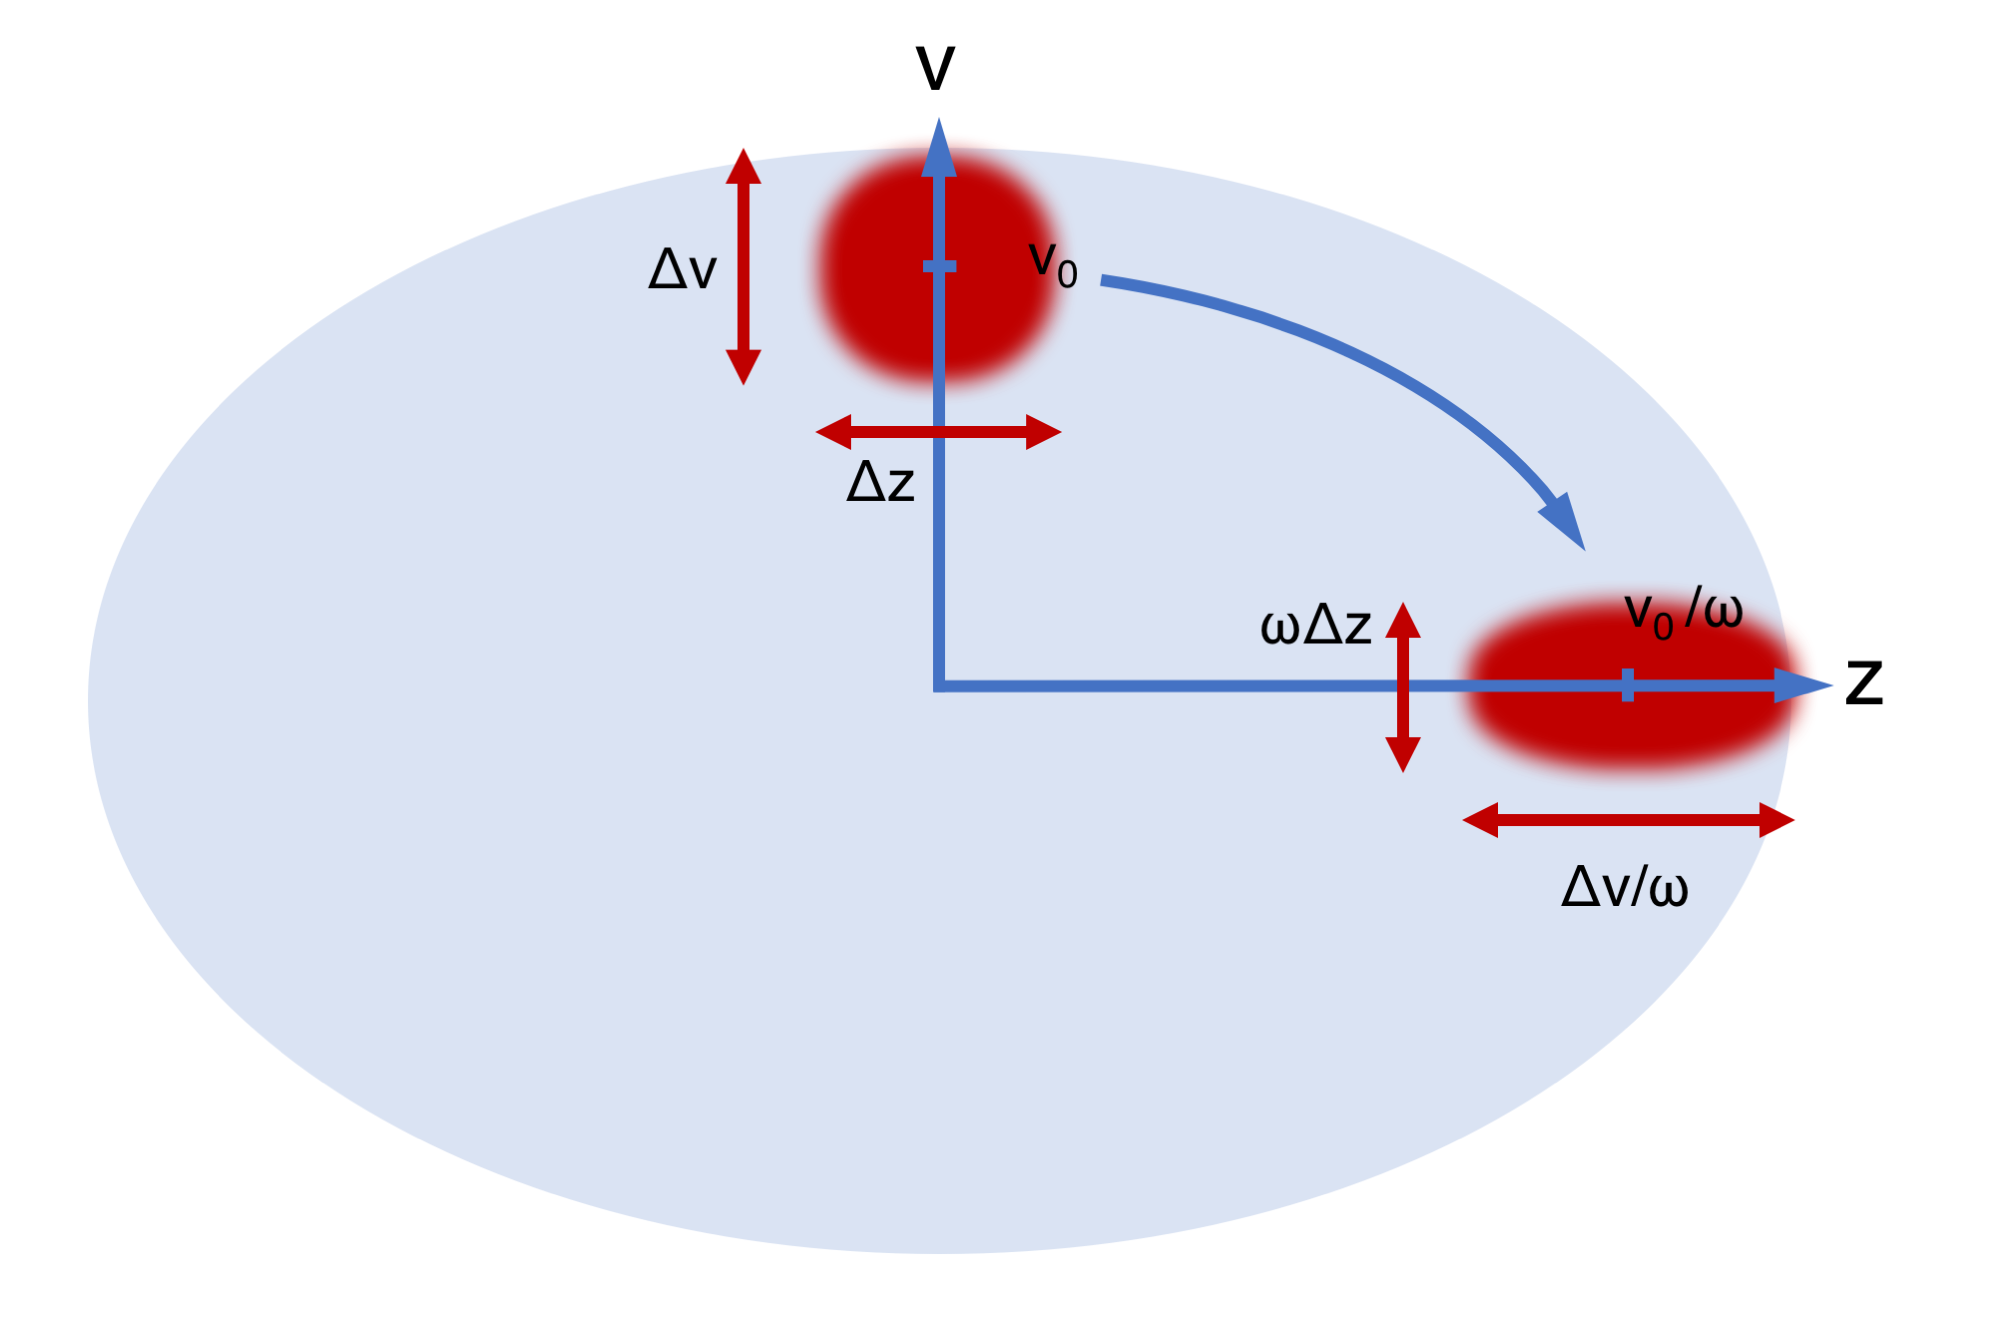
\includegraphics[width=10cm]{LoadingRotation.png}
\caption[Ideal Trap Loading as a Quarter Rotation]{\label{LoadingRotation}
Phase space diagram depicting the action of the ideal phase space conservative loading fields derived from a large external harmonic potential. The region of phase space acted on by the external potential is indicated as a light blue ellipse. The region of phase space populated initially is shown in red along the $v$ axis. The region populated after rotation is shown along the $z$ axis also in red. Widths and origins are as indicated.
}
\end{figure}

In addition to this harmonic loading potential, it would be ideal to also maintain a transverse trap simultaneously. 
The ideal fields would have a magnitude with the following spatial dependence:
\begin{equation}
|E(x,y,z)| = \frac{1}{2}m_{OH}\left(\omega_z^2z^2 + \omega_r^2r^2\right)
\end{equation}
where $\omega_z$ and $\omega_r$ are the longitudinal and transverse trap frequencies.
Neglecting the nonlinearity of the Stark shift for OH molecules close to zero field, such a harmonic potential could be generated transversely with a hexapole, but to do it simultaneously in the transverse and longitudinal directions would require an octupole moment, such as could be generated with three rings and two endcaps with the endcaps at $+V$, the outer rings grounded, and the inner one at $-V/2$ so as to approximate spherical boundary conditions following the second Legendre polynomial~\cite{jackson1999classical}.
This would of course be very unlikely to be able to be crammed into the small space between the end of a decelerator and a trap, and unlikely to be able to be charged up to a high enough potential energy for stopping an appreciable speed $v$.

It is much more likely that an efficient solution would be obtained by abandoning the harmonicity and instead focusing on the reduced criterion of loading fields that respect phase stability by having a slope at the location of what will be come the trap center and which also provide some transverse confinement.
The slope of the loading field at the location of the trap center would ideally match the slope that the ideal harmonic trap with frequency $\omega$ would have at that point, $m_{OH}\omega v_0$.

\begin{figure}[t!]
\centering
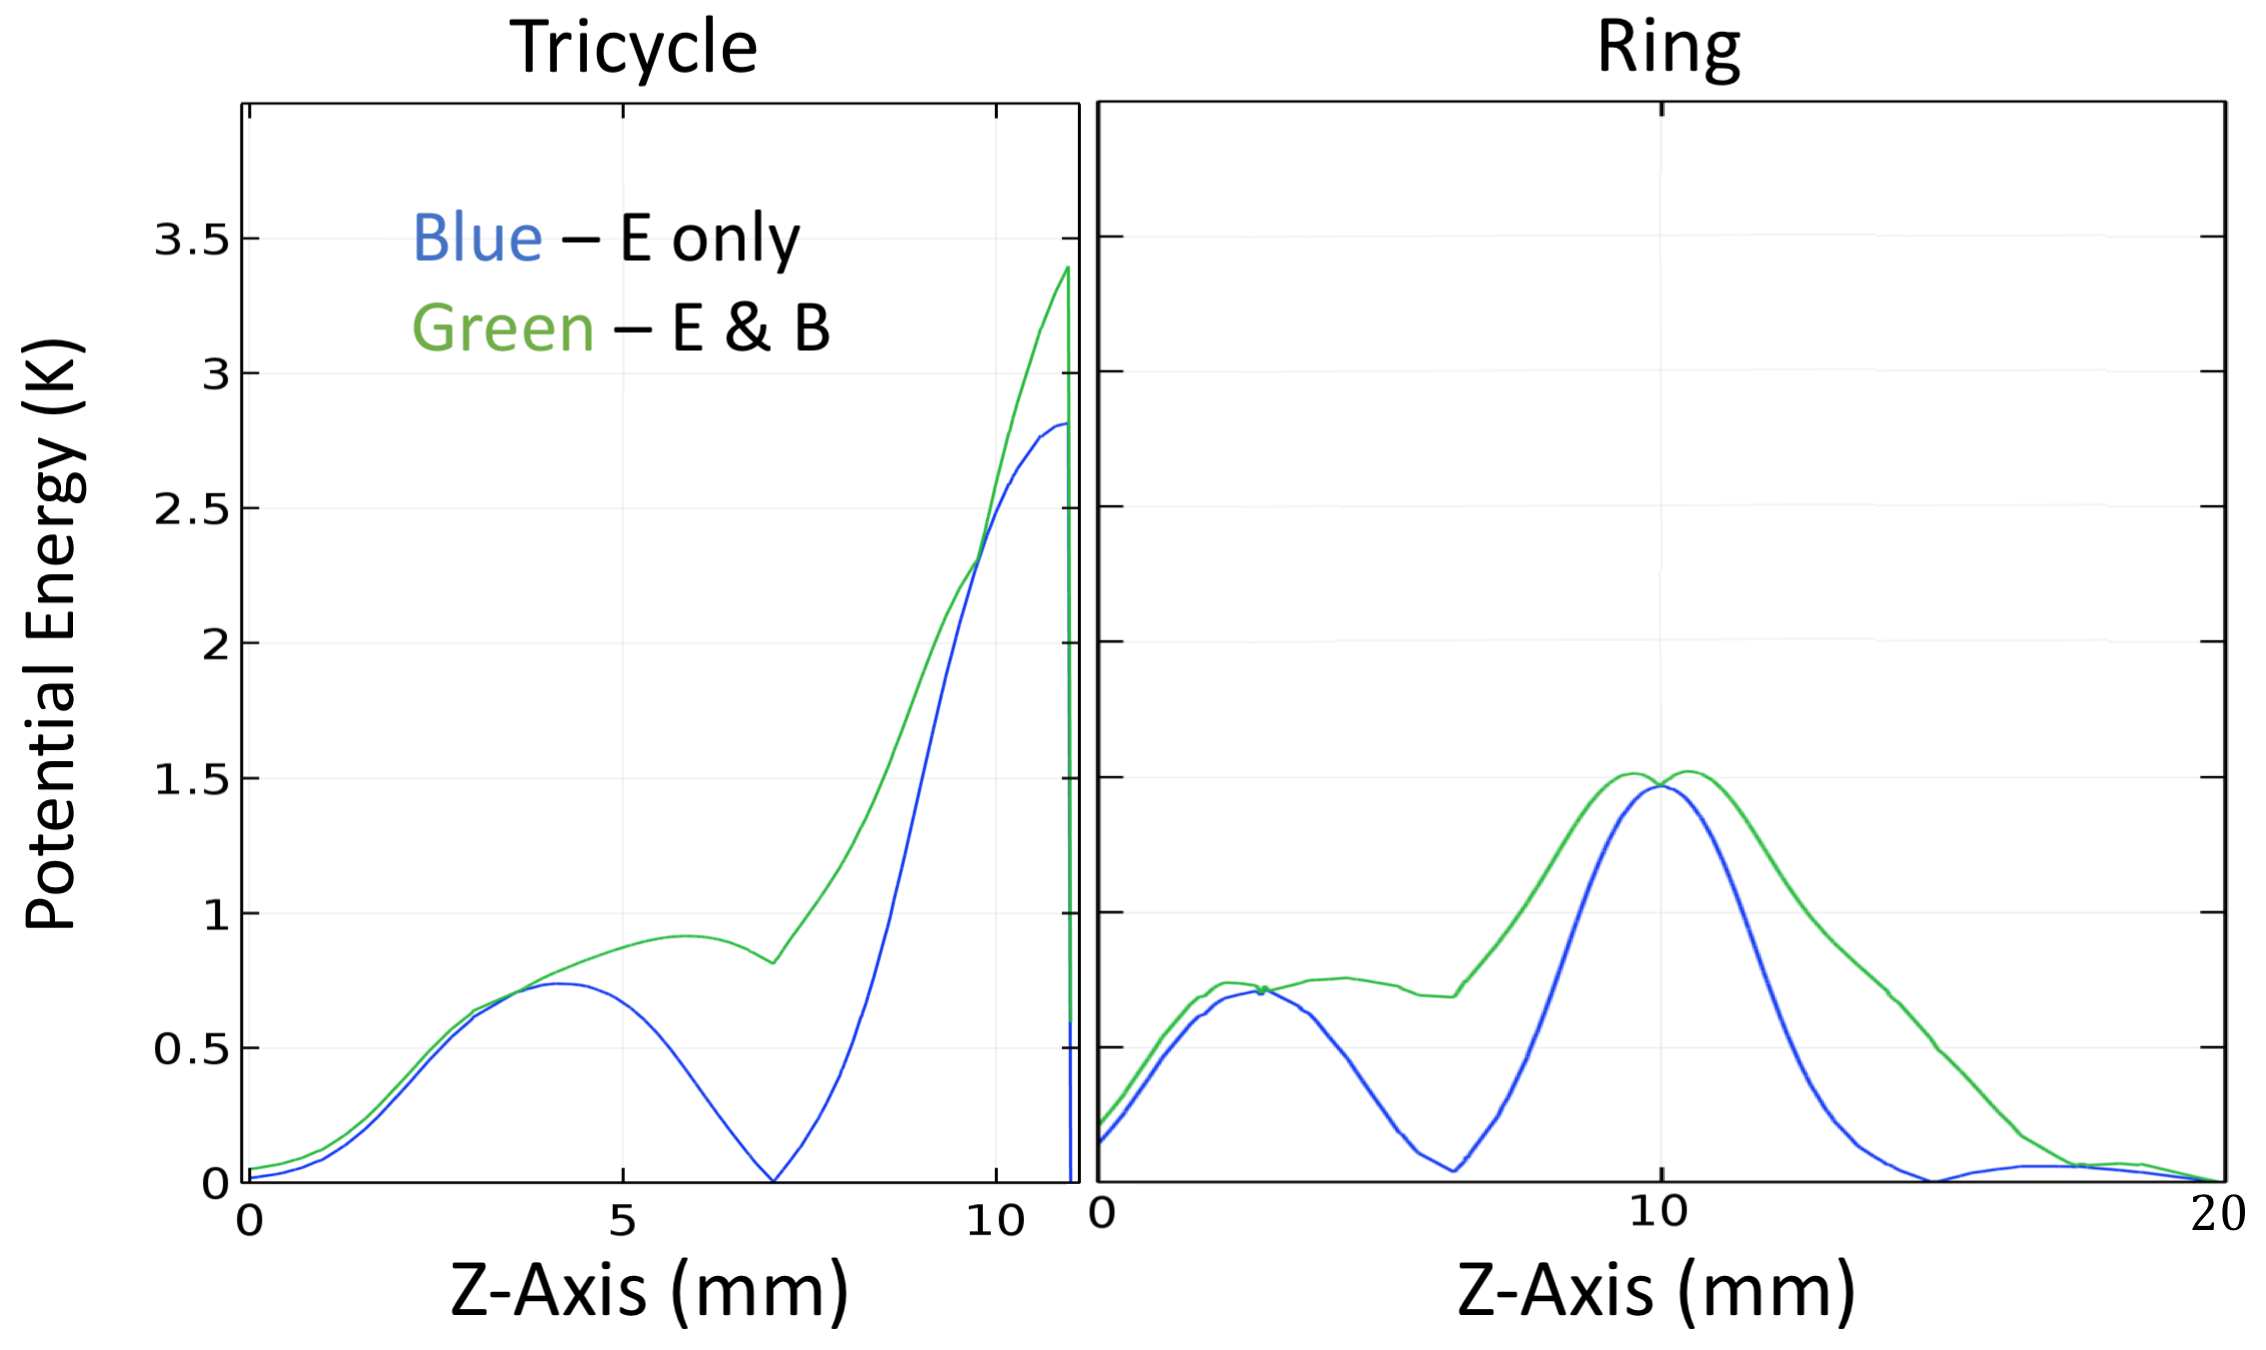
\includegraphics[width=14cm]{LoadingFieldsEB.png}
\caption[On-Axis Loading for Ring and Tricycle]{\label{loadingringtrike}
Potential energy along axis for Ring and Tricycle traps. The trap center is located at $z=10$~mm in both cases. Note the more favorable slope of the loading potential in the vicinity of the trap center for the tricycle trap. Field magnitudes arise from application of $\pm12.5\text{ kV}$ for the Ring trap and also for the Tricycle. In practice almost half this voltage was applied on the Tricycle for optimal operation, perhaps due to arcing effects or nonadiabatic transitions during loading discussed below in Sec.~\ref{loadingtransitions}.
}
\end{figure}

In practice, Fig.~\ref{loadingringtrike} shows what we are able to obtain for loading fields comparing the Ring and Tricycle traps.
Note the role of the magnetic field, which is non-negligible.
The tricycle trap comes much closer to the harmonic ideal discussed above.
For the ring trap, the extra effect of the magnetic field actually depresses the potential energy at the trap center below a wider plateau, making it formally impossible to bring the synchronous molecule to rest at the trap center.
In practice, the experimentally determined ideal application time of loading fields likely corresponds to the synchronous molecule bringing brought close to rest but out in front of the trap center.

This unideal situation should result in a higher loaded temperature in the ring trap compared with the tricycle trap, $87$~mK compared with $61$~mK in simulation.
In practice however, the measured spectra of molecules in the Ring trap fits better to a thermal distribution and to a lower temperature compared with the tricycle trap.

\subsection{Loaded Spectra}

\figdave{RingTriSpectrum.png}{Spectra in Ring and Tricycle Trap}{Spectra in the Ring and Tricycle traps after loading with no evaporation. The former was published in \citep[Fig.~3a]{stuhl2012evap}, the latter was collected on Feb.~24, 2014.}{\linewidth}

The obtained spectra in the two traps are compared in Fig.~\ref{ringtricyclespectra}.
Several important features are worth discussing here.
First of all, the ring trap fits nicely to a Maxwell-Boltzmann distribution, which in a linear trapping geometry should scale with magnetic field in the following way:
\begin{equation}
p(B)\propto B^2e^{\mu_B B/kT}.
\end{equation}
The exponential term gives the expected Boltzmann suppression factor as a function of increasing potential energy, while the $B^2$ term is proportional to the volume degeneracy factor.
In other words, the volume corresponding to a magnetic field $B$ within $dB$ is an ellipsoidal shell in the linear trap, whose surface area grows proportionally to $B^2$ since the trap is linear.
However, this simple picture should be completely violated in the ring trap by the time one approaches the barrier between the central ring trap and its toroidal outer trap, at which point the linearity of the trap is invalid.
If molecules were thermally exploring this region, there ought to be a large peak in the ring trap spectra corresponding to the plateaus evident close to $1100$~G.




\section{Trap Loading}

\section{Spin-Flips During Loading}
\label{loadingtransitions}

\section{Pin Trap}

\section{Other traps in the field}

\section{Spin-flip Losses, Dipolar Enhancements thereof}

\section{Dynamical Phenomenon}

\section{Next Generation Traps}



\bibliographystyle{unsrtDR}	% or "siam", or "alpha", etc.
\bibliography{allrefs}		% Bib database in "allrefs.bib"
\end{document}




